% Indice
\tableofcontents
\newpage

%% Capitulo 1
\thispagestyle{empty}
\part{Ecuaciones Diferenciales Ordinarias con más de dos Variables}

En este capítulo se estudiarán conceptos básicos para la solución de ecuaciones diferenciales parciales, para lo cual se recolectan conceptos de geometría y ecuaciones diferenciales ordinarias.

\section{Superficies y Curvas en Tres Dimensiones}

Tomando una superficie en el espacio cartesiano $(x,y,z)$
	$$f(x,y,z) = 0$$
Se escoje un punto que satisface la ecuación anterior y se incrementa $(\delta x, \delta y, \delta z)$ lo que esta relacionado con la ecuación
	$$\pdv{f}{x} \delta x + \pdv{f}{y} \delta y + \pdv{f}{z} \delta z = 0$$
En otras palabras, en la vecindad de $P(x,y,z)$ existen puntos $P'(x + \xi ,y + \eta , z + \zeta)$ que satisfacen la ecuación de superficie y que para cualesquiera dos, el tercero esta dado por:
	$$\xi \pdv{f}{x} + \eta \pdv{f}{y} + \zeta \pdv{f}{z} = 0$$
	
Las ecuaciones de la forma:
	$$x = F_1 (u,v) \quad \quad y = F_2 (u,v) \quad \quad z = F_3 (u,v)$$
Son conocidas como las \textbf{Ecuaciónes Paramétricas de la Superficie.} Esto es porque tanto $u$ como $v$ pueden ser expresadas como funciones de $x$ e $y$, una vez se encuentre dichos valores, se conocerán $u$ y $v$; además, $z$ se encuentra sustituyendo lo encontrado anteriormente en su ecuación, con esto, es claro que cumplen con la ecuación de superficie. \\

Cabe recalcar que varios conjuntos de ecucaciones paramétricas generan las mismas superficies, vease:
	$$(a\sin{u} \cos{v} , a\sin{u} \cos{v} ,a\cos{u})$$
Y 
	$$\qty(a\frac{1 - v^2}{1 + v^2} \cos{u} , a\frac{1 - v^2}{1 + v^2} \sin{u} ,\frac{2av}{1 + v^2})$$

Generan la superficie esférica
	$$x^2 + y^2 + z^2 = a^2$$
	
Las superficies pueden ser previstas como una curva, siempre y cuando cumplan con las ecuaciones de la superficie y esten en el plano $z = k$. Lo que significa que $(x,y,z)$ esta en la curva $\Gamma _k$.

Tomando como ejemplo:

\begin{figure}[H]
	\centering
	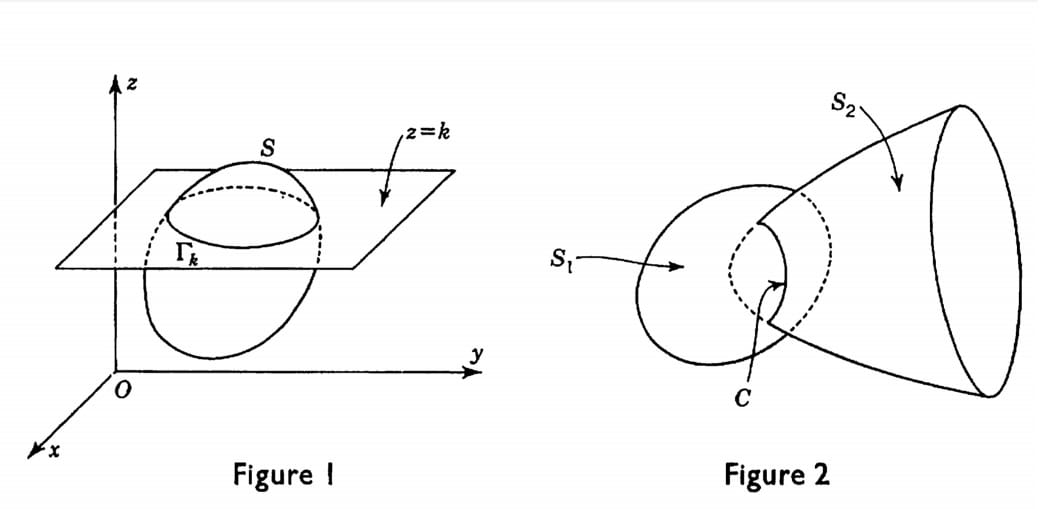
\includegraphics[scale=0.45]{Images/surfaceSection1.jpeg}
	\caption{Ejemplo de Curva en Superficie}
	\label{curveSurface}
\end{figure}

Esta idea puede ser facilmente generalizada simplemente tomando dos superficies que se intersectan, la curva de intersección es el análogo de $\Gamma _k$ en el ejemplo anterior. Esta idea esta representada en la "Figure 2" de \ref{curveSurface}. Matemáticamente hablando, la curva $C$ es conformada por todos aquellos puntos que cumplen las ecuaciones de ambas superficies:
	$$f(x,y,z) = 0 \quad \quad g(x,y,z) = 0$$
Dicha curva se puede representar por medio de sus ecuaciones paramétricas. Ahora, suponiendo que la curva $C$ esta sobre la superficie cuya ecuación es:
	$$F(x(t),y(t),z(t)) = 0$$
Derivando $F$ se tienen la relación:
	$$\pdv{F}{x} \dv{x}{t} + \pdv{F}{y} \dv{y}{t} + \pdv{F}{z} \dv{z}{t} = 0$$
De modo que la tangente a la curva es:
	$$\qty(\pdv{F}{x} , \pdv{F}{y} , \pdv{F}{z})$$
	
La ecuación del plano $\pi _1$ en el punto $P(x,y,z)$ y la superficie $S_1$ es:
	$$(X - x)\pdv{F}{x} + (Y - y)\pdv{F}{y} + (Z - z)\pdv{F}{z} = 0$$
Con $(X,Y,Z)$ es cualquier otro punto en el plano. Realizando lo mismo para la superficie $S_2$. Se tiene:
	$$(X - x)\pdv{G}{x} + (Y - y)\pdv{G}{y} + (Z - z)\pdv{G}{z} = 0$$
Y la intersección $L$ de los planos $\pi _1$ y $\pi _2$ en $P$ es tangente a la curva $C$. \\

Para visualizarlo de mejor manera, se tiene la siguiente figura:

\begin{figure}[H]
	\centering
	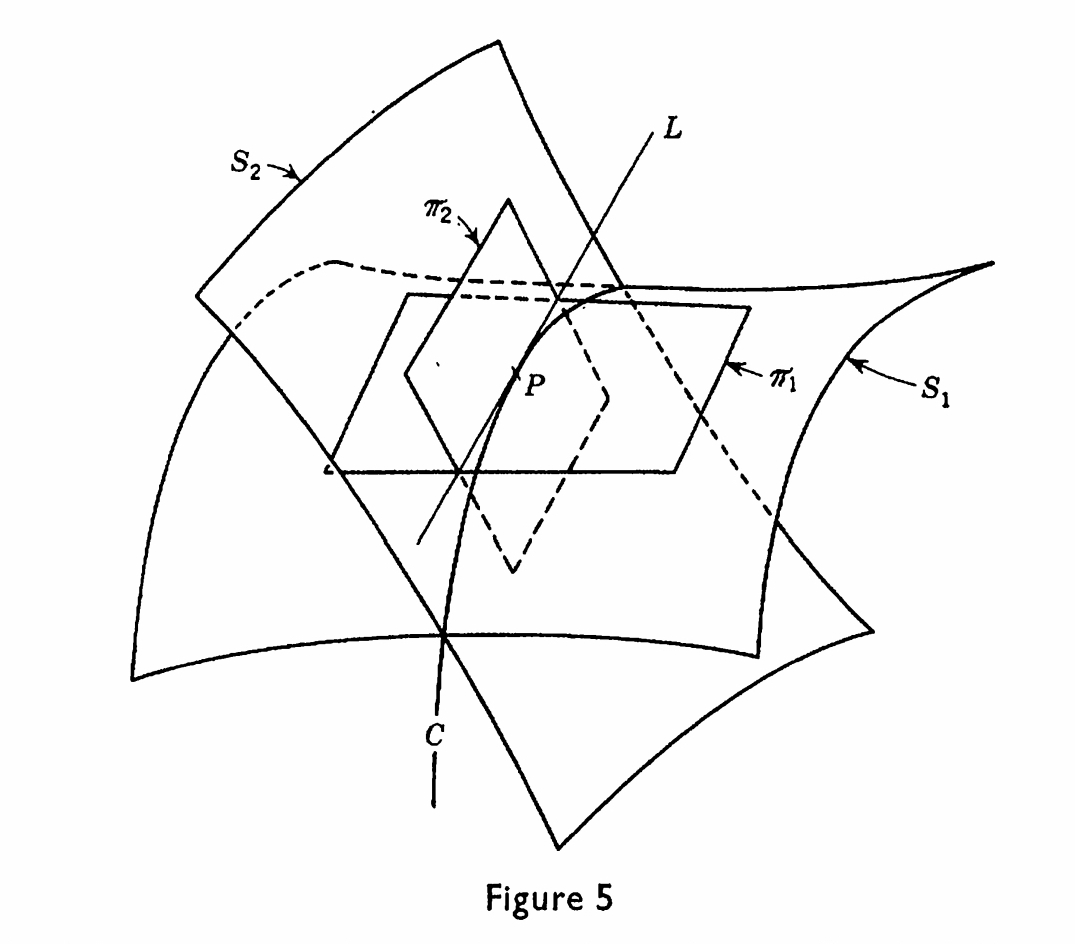
\includegraphics[scale=0.2]{Images/planesSection1.jpeg}
	\caption{Visualización de la Recta Tangente a la Curva}
	\label{planes}
\end{figure}

De las ecuaciones de los planos se tiene que las ecuaciones de la recta $L$ son:
	$$\frac{X - x}{\pdv{F}{y} \pdv{G}{z} - \pdv{F}{z} \pdv{G}{y}} = \frac{Y - y}{\pdv{F}{z} \pdv{G}{x} - \pdv{F}{x} \pdv{G}{z}} = \frac{Z - z}{\pdv{F}{x} \pdv{G}{y} - \pdv{F}{y} \pdv{G}{x}}$$

En otras palabras, las razones de dirección de la recta $L$ son:
	$$\Bigg\{ \pdv{(F,G)}{(y,z)} , \pdv{(F,G)}{(z,x)} , \pdv{(F,G)}{(x,y)} \Bigg\}$$


\subsection{Problemas Resueltos}


\section{Ecuaciones Diferenciales de Primer Orden y Primer Grado de Tres Variables}

Un ejemplo claro de sistema de ecuaciones simultaneas de primer orden y primer grado es:
	$$\dv{x_i}{t} = f_i (x_1 ,\ldots ,x_n ,t)$$
aparece frecuentemente en física. Otro ejemplo claro, es el Hamiltoniano de un sistema en movimiento con $n$ grados de libertad tiene la forma:
	$$\dv{p_i}{t} = -\pdv{H}{q_i} \quad \quad \dv{q_i}{t} = \pdv{H}{p_i} \quad \quad i = 1,\ldots ,n$$
Donde $H(q_1,\ldots ,q_n ,p_1,\ldots ,p_n ,t)$ es el Hamiltoneano del sistema. Para un sistema de un grado de libertad se tiene:
	$$\dv{p}{t} = -\pdv{H}{q} \quad \quad \dv{q}{t} = \pdv{H}{p}$$
Si se tiene:	
	$$-\pdv{H}{q} = \frac{P(p,q,t)}{R(p,q,t)} \quad \quad \pdv{H}{p} = \frac{Q(p,q,t)}{R(p,q,t)}$$
La ecuación anterior se puede colocar de la forma:
	$$\frac{\dd{p}}{P(p,q,t)} = \frac{\dd{q}}{Q(p,q,t)} = \frac{\dd{t}}{R(p,q,t)}$$
Dado esto, la ecuación anterior se puede expresar de una forma general, teniendo $P,Q,R$ funciones de $x,y,z$, entonces se tiene:

\begin{align}
	\frac{\dd{x}}{P} = \frac{\dd{y}}{Q} = \frac{\dd{z}}{R} \label{formaPQR}
\end{align}

Para asegurar la unicidad de la ecuación se tiene el siguiente teorema:

\begin{teorema} \it
	Si las funciones $f_1 (x,y,z)$ y $f_2 (x,y,z)$ son continuas en una región definida por $\abs{x - a} < k$, $\abs{y - b} < l$, $\abs{z - c} < m$ y si en dicha región las funciones satisfacen una condición Lipschitz del tipo:
		$$\abs{f_1 (x,y,z) - f_1 (x,\eta ,\zeta)} \leq A_1 \abs{y - \eta} + B_1 \abs{z - \zeta}$$
		$$\abs{f_2 (x,y,z) + f_2 (x,\eta ,\zeta)} \leq A_2 \abs{y - \eta} + B_2 \abs{z - \zeta}$$
	en un intervalo adecuado $\abs{x - a} < h$ existe un único par de funciones $y(x)$ y $z(x)$ continuas y con derivadas continuas en dicho intervalo, que satisfacen las siguientes ecuaciones diferenciales:
		$$\dv{y}{x} = f_1 \quad \quad \dv{z}{x} = f_2$$
	y que tienen la propiedad de $y(a) = b$, $z(a) = c$ donde $a,b,c$ son arbitrarios.
\end{teorema}

No se demostrará este teorema, para una demostración formal consulte el siguiente libro de análisis\footnote{E. Goursat, "A Course in Mathematical Analysis" (Ginn, Boston, 1917), vol. II, pt. II, pp. 45ff.}. \\

El resultado del teorema se muestra en la figura \ref{teorem1Figure}. En base al teorema, existe un cilindro $y = y(x)$ pasando por el punto $(a,b,0)$, y un cilindro $z = z(x)$ pasando por le punto $(a,0,c)$, tales que $\dv{y}{x} = f_1$ y $\dv{z}{x} = f_2$. La solución completa del par de ecuaciones consiste en un conjunto de puntos en común con los cilindros, es decir, la curva de intersección $\Gamma$.

\begin{figure}[H]
	\centering
	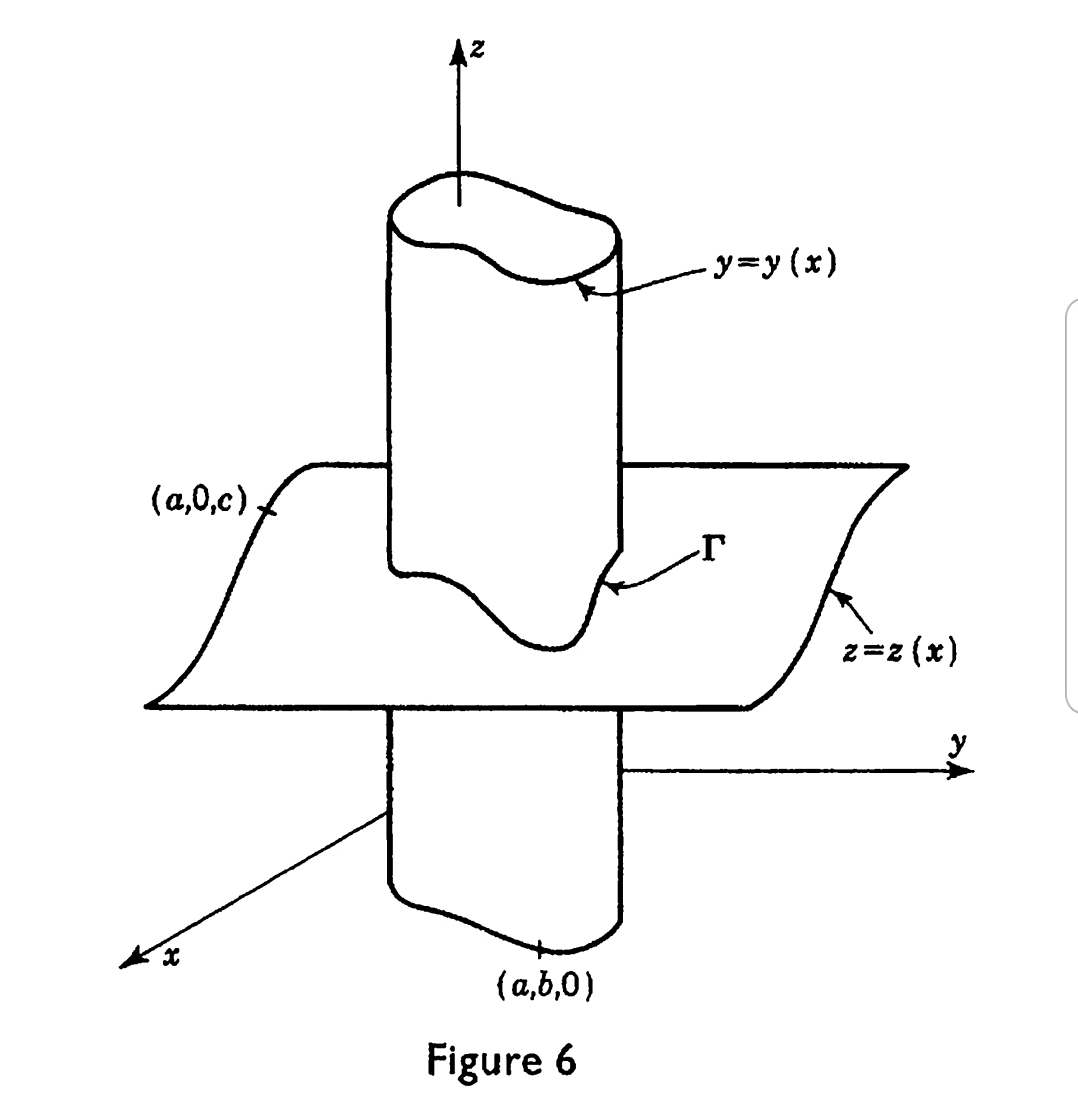
\includegraphics[scale=0.15]{Images/teorem1Figure.jpeg}
	\caption{Visualización del Teorema $1$}
	\label{teorem1Figure}
\end{figure}

De esto se concluye que, la solución general del conjunto de ecuaciones del tipo \eqref{formaPQR} será una familia de curvas de dos parámetros.

\subsection{Métodos de Solución de $\flatfrac{\dd{x}}{P} = \flatfrac{\dd{y}}{Q} = \flatfrac{\dd{z}}{R}$}


De la sección anterior se tiene:
	$$\frac{\dd{x}}{P} = \frac{\dd{y}}{Q} = \frac{\dd{z}}{R}$$
Si se pueden derivar dos relaciones de la forma:
	$$u_1 (x,y,z) = c_1 \quad \quad u_2 (x,y,z) = c_2$$
Variando esas constantes, se obtiene la familia de curvas que satisfacen la ecuación. \\

\textit{Método (a): } Para encontrar las funciones $u_1$ y $u_2$ se puede observar que cualquier dirección tangencial por un punto $(x,y,z)$ a una superficie $u_1 = c_1$ satisface la relación:
	$$\pdv{u_1}{x} \dd{x} + \pdv{u_1}{y} \dd{y} + \pdv{u_1}{z} \dd{z} = 0$$

Si $u_1 = c_1$ es un sistema adecuado de superficies, la dirección tangencial a la curva de integral por el punto $(x,y,z)$ si también es una dirección tangencial a esta superficie. De esto:
	$$P\pdv{u_1}{x} + Q\pdv{u_1}{y} + R\pdv{u_1}{z} = 0$$
Para encontrar $u_1$, y similarmente $u_2$, se intenta encontrar funciones $P'$, $Q'$ y $R'$ tales que:
	\begin{align}
		PP' + QQ' + RR' = 0 \label{PPQQRR}
	\end{align}
Y, además, existe una función $u_1$ con las propiedades:
	$$P' = \pdv{u_1}{x}, \quad \quad Q' = \pdv{u_1}{y},\quad \quad R' = \pdv{u_1}{z}$$
Lo que implica que:
	$$P' \dd{x} + Q'\dd{y} + R'\dd{z}$$
Es una diferencial exacta de $\dd{u_1}$. Se tomará el ejemplo $2$ del libro (Sección $3$, capítulo $1$, pp. 11.)

\begin{ejemplo} \slshape
	Encuentre las curvas de integral de las ecuaciones:
		$$\frac{\dd{x}}{y(x + y) + az} = \frac{\dd{y}}{x(x + y) - az} = \frac{\dd{z}}{z(x + y)}$$
	En este caso se tiene:
		$$P = y(x + y) + az \quad \quad Q = x(x + y) - az \quad \quad R = z(x + y) $$
	Tomando
		$$P' = \frac{1}{z} \quad \quad Q' = \frac{1}{z} \quad \quad R' = -\frac{x + y}{z^2}$$
	La condición \eqref{PPQQRR} se satisface, entonces:
		$$u_1 = \frac{x + y}{z}$$
	Similarmente, si se toma:
		$$P' = x \quad \quad Q' = -y \quad \quad R' = -a$$
	la condición \eqref{PPQQRR} se satisface, la función correspondiente:
		$$u_2 = \frac{1}{2} (x^2 - y^2) - az$$
	De modo que las curvas de integral para las ecuaciones diferenciales son la familia de dos parámetros:	
		$$x + y = c_1 z \quad \quad x^2 - y^2 - 2az = c_2$$
\end{ejemplo}



\textit{Método (b): } Suponga que se pueden encontrar tres funciones $P',Q',R'$ tal que:
	$$\frac{P' \dd{x} + Q' \dd{y} + R'\dd{z}}{PP' + QQ' + RR'}$$
Es un diferencial exacto $\dd{W'}$, y si se pueden encontrar otras tres funciones $P'',Q'',R''$ tales que:
	$$\frac{P'' \dd{x} + Q'' \dd{y} + R''\dd{z}}{PP'' + QQ'' + RR''}$$
El cual es un diferencial exacto $\dd{W''}$. De esto, se sabe que:
	$$\dd{W'} = \dd{W''}$$
De lo que se deriva.
	$$W' = W'' + c_1$$
Donde $c_1$ es una constante arbitraria.


\begin{ejemplo} \slshape
	Utilizando el método \textit{(b)}, se resuelven las ecuaciones:
		$$\frac{\dd{x}}{y + \alpha z} = \frac{\d{y}}{z + \beta x} = \frac{\dd{z}}{x + \gamma y}$$
	Reescribiendo la ecuación como en el método se tiene
		$$\frac{\lambda \dd{x} + \mu \dd{y} + \nu \dd{z}}{\lambda (y + \alpha z) + \mu (z + \beta x) + \nu (x + \gamma y)}$$
	
\end{ejemplo}



  	























